% Example LaTeX document  - note % sign indicates a comment
\documentclass[11pt]{article}
% Default margins are too wide all the way around.  You can reset them here
\setlength{\topmargin}{-.5in}
\setlength{\textheight}{9in}
\setlength{\oddsidemargin}{.125in}
\setlength{\textwidth}{6.25in}

\usepackage{graphicx}  % for insert images

\begin{document}
\title{SCI 101-04 Homework 2}
\author{Olivia Stopka\\
Manhattan College}
\renewcommand{\today}{February 5, 2019}
\maketitle
This is the Homework Assignment Part 1



\section{Section 1}
 Career Goal:
 When I graduate from Manhattan College, I hope to be a successful woman in the work force of computer science. I hope to be working in the field of cyber security. 



\section{Section 2 School ID}
\begin{figure}[!h]
\center{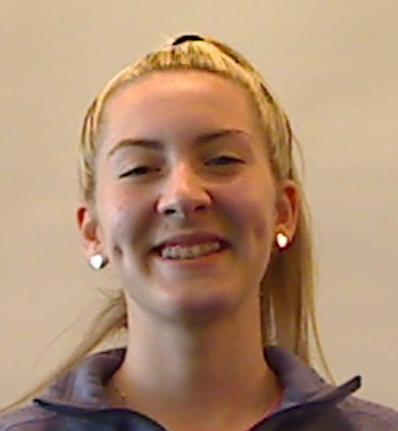
\includegraphics[width=0.2\textwidth] {pic_olivia}} 
\end{figure}



\section{Table}
\begin{table}[h]
\caption{Multiplication Table}
\centering
\begin{tabular}{ |c|c|c|c|c|c|c|c|c|c|}
\hline
     & 1 & 2 & 3& 4 & 5& 6 & 7& 8 &9 \\
     \hline

          & 2 & 4 & 6& 8 & 10& 12 & 14& 16&18 \\
          \hline

               & 3 & 6 & 9& 12 & 15& 18 & 21& 24 &27 \\
\hline
     & 4 & 8 & 12& 16 & 20& 24 & 28& 32 &36 \\
\hline
     & 5 &10 & 15& 20 & 25& 30 & 35& 40 &45 \\
\hline
     & 6 & 12 & 18& 24 & 30& 36 & 42& 48 &54\\
\hline
 & 7 & 14 & 21& 28 & 35& 42 & 49& 56 &63 \\
\hline
 & 8 & 16 & 24& 32 & 40& 48 & 56& 64 &72 \\
\hline
 & 9 & 18 & 27& 36 & 45& 54 & 63& 72 &81 \\
\hline
 \end{tabular}
\end{table}




\section{ Math Equation}

\[x=\frac{-b\pm \sqrt{b^{2}-4ac}}{2a}\]

\end{document}









